%!TEX root = ../template.tex

%%%%%%%%%%%%%%%%%%%%%%%%%%%%%%%%%%%%%%%%%%%%%%%%%%%%%%%%%%%%%%%%%%%%%%%%%%%%%%%%

\section{Physical human-robot interaction in Gazebo: lifting the iCub arm}

To test the control software for the robot lifting with the help of the human, we first realized a prototype application in Gazebo. In this application, the robot can lift from a chair autonomously or with the help of a human; to realize a physical interaction between the human (operator, in this case) and the robot simulated in Gazebo, we used the Geomagic touch, a haptic device.

The setup consists of:
\begin{itemize}
\item the iCub simulation in Gazebo, complete of the dynamics information provided by \textit{wholeBodyDynamicsTree} (\url{https://github.com/robotology/codyco-modules/tree/master/src/modules/wholeBodyDynamicsTree} developed by IIT in WP1) and the Cartesian information provided by \textit{iKinCartesianController};
\item the Geomagic Touch, installed following the instructions in \url{https://github.com/inria-larsen/icub-manual/wiki/Installation-with-the-Geomagic-Touch}, which not only install the SDK and drivers of the GeoMagic but also point to how to create the yarp drivers for the Geomagic;
\item a C++ module (\url{https://github.com/inria-larsen/icubLearningTrajectories}) that connects the output command from the Geomagic to the iCub in Gazebo, and eventually enables recording the trajectories on a file.
\end{itemize}

The interconnection among the different modules is sketched in Figure~\ref{fig:systemHaptic}.
The tip of the Geomagic is virtually attached to the end-effector of the robot:
$$ x_{geo} \rightarrow x_{icub\_hand} $$
When the operator moves the Geomagic in the space, the position of the Geomagic tip $x_{geo}$ is scaled (1:1 by default) in the iCub workspace as $x_{icub\_hand}$, and the Cartesian controller is used to move the iCub hand around a "home" position, or default starting position:
$$ x_{icub\_hand} = hapticDriverMapping(x_0 + x_{geo})$$
where the \textit{hapticDriverMapping} is the transformation applied by the haptic device driver, which basically maps the axis from the Geomagic reference frame to the iCub reference frame.
By default, no force feedback is sent back to the operator in this mode, as it emulates the zero-torque control pHRI where the robot is ideally transparent and not opposing any resistance to the human guidance. A default orientation of the hand ("katana" orientation) is set.

\begin{figure}[h]
\centering
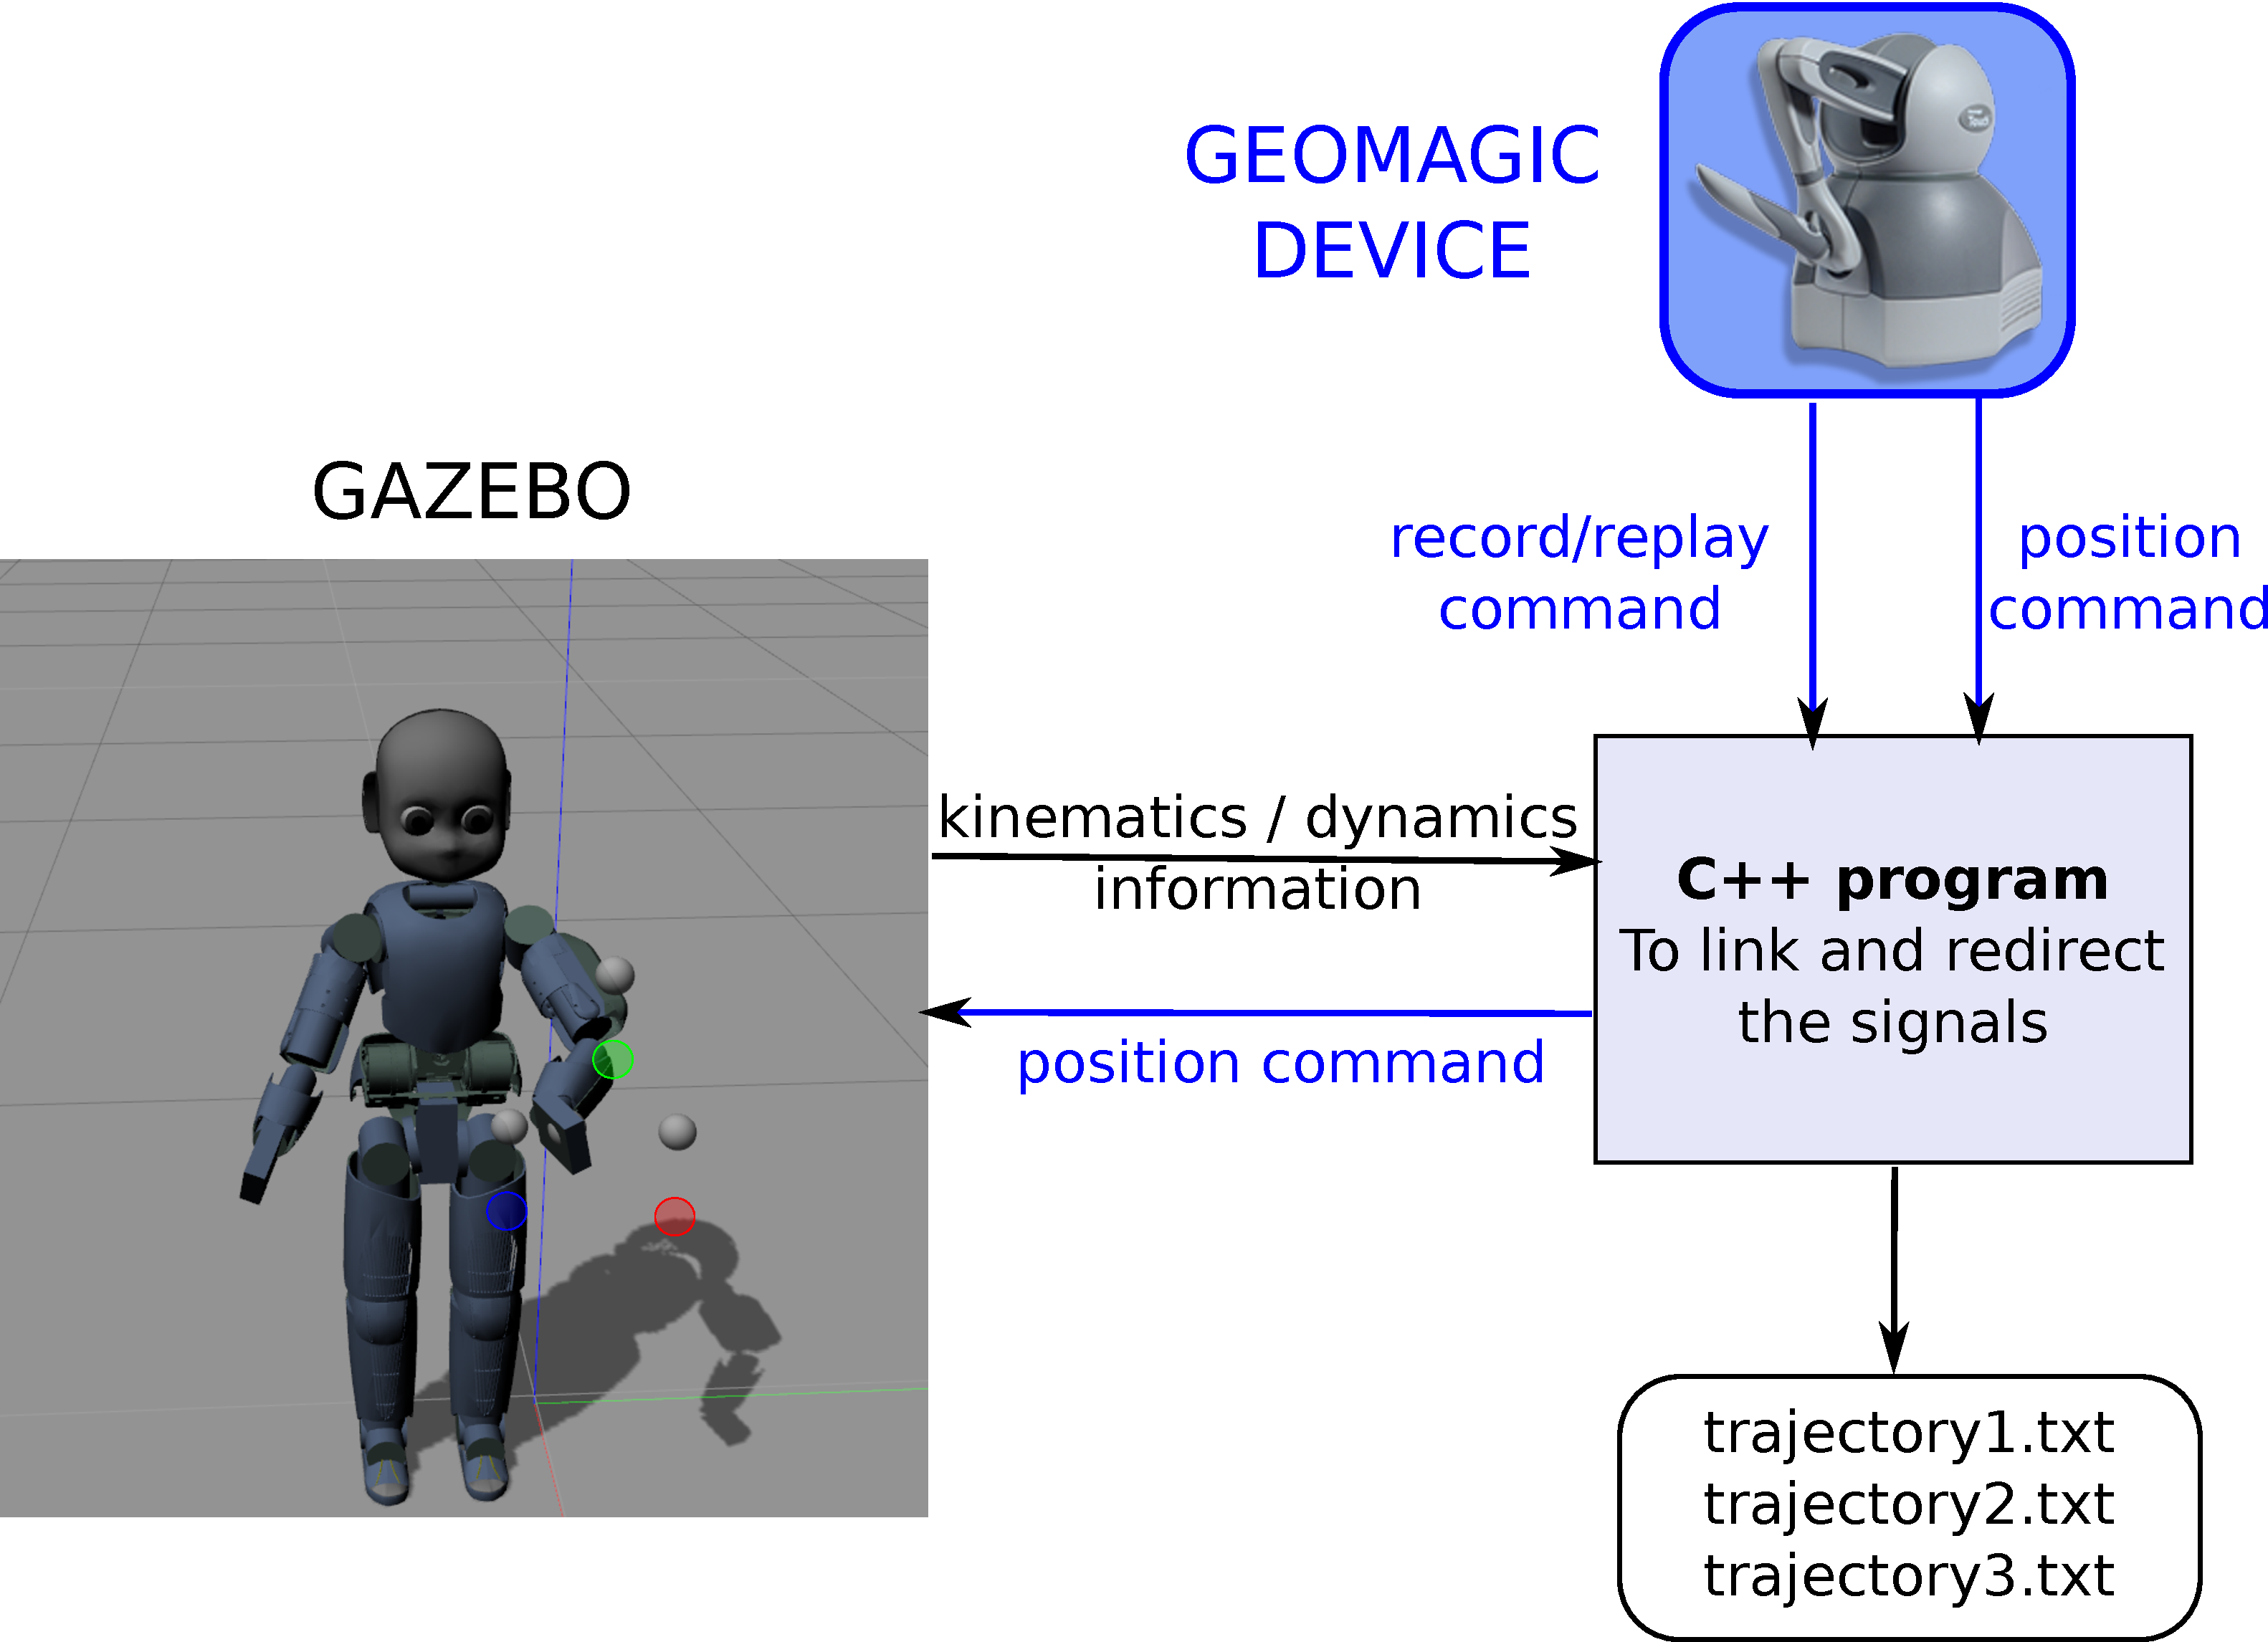
\includegraphics[height=7cm]{figs/geomagic_setup.pdf}
\caption{The interconnection between the Geomagic Touch and iCub in Gazebo.}
\label{fig:systemHaptic}
\end{figure}

The two buttons of the Geomagic are used to enable recording and replaying the trajectories (see Figure~\ref{fig:geobuttons}). To record a trajectory, the operator must click and hold the black button of the Geomagic; releasing the button stops recording the trajectory, and the trajectory is saved on a file (e.g., \textit{trajectory.txt}). To replay one of the trajectories from the $N$ previously recorded, the operator must click the light grey button of the Geomagic and then enter the number of the trajectory on the terminal.

\begin{figure}[h]
\centering
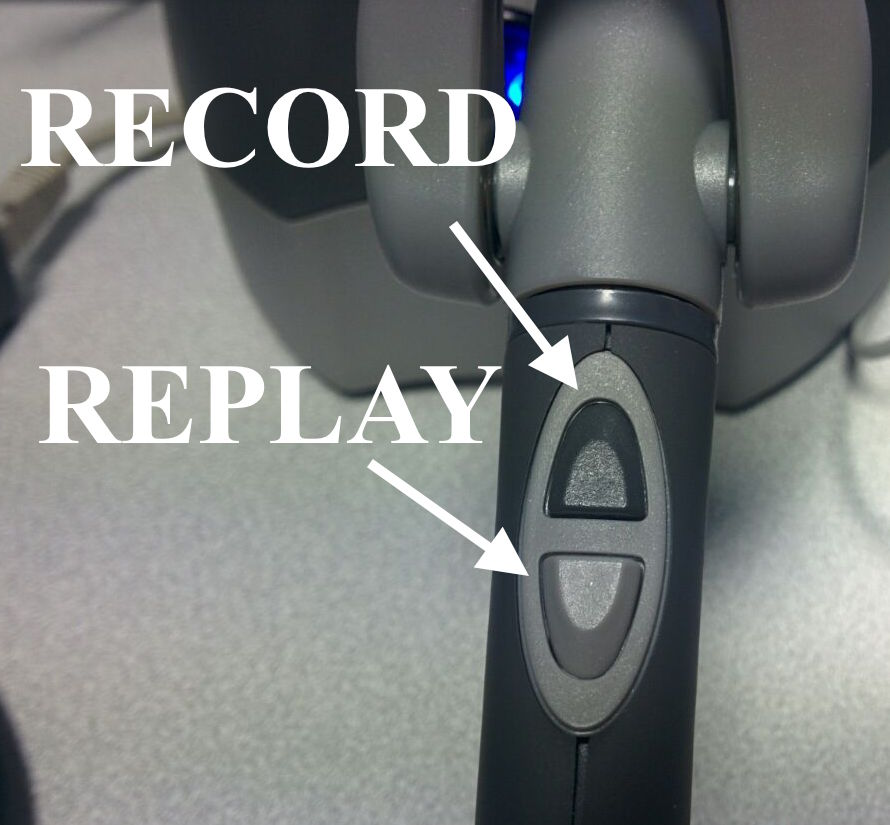
\includegraphics[height=5cm]{figs/geomagic_buttons.jpg}
\caption{The two buttons of the Geomagic.}
\label{fig:geobuttons}
\end{figure}

A video showing the iCub moved by the haptic device in Gazebo is available at this link: \url{https://www.youtube.com/watch?v=4ShyNtKojy0&feature=youtu.be}.
The graph in Figure~\ref{fig:trajectories} shows some trajectories recorded from the geomagic, corresponding to lifting the left arm of the iCub: the Cartesian position of the hand in the reference frame of iCub is shown.
\begin{figure}[h]
\centering
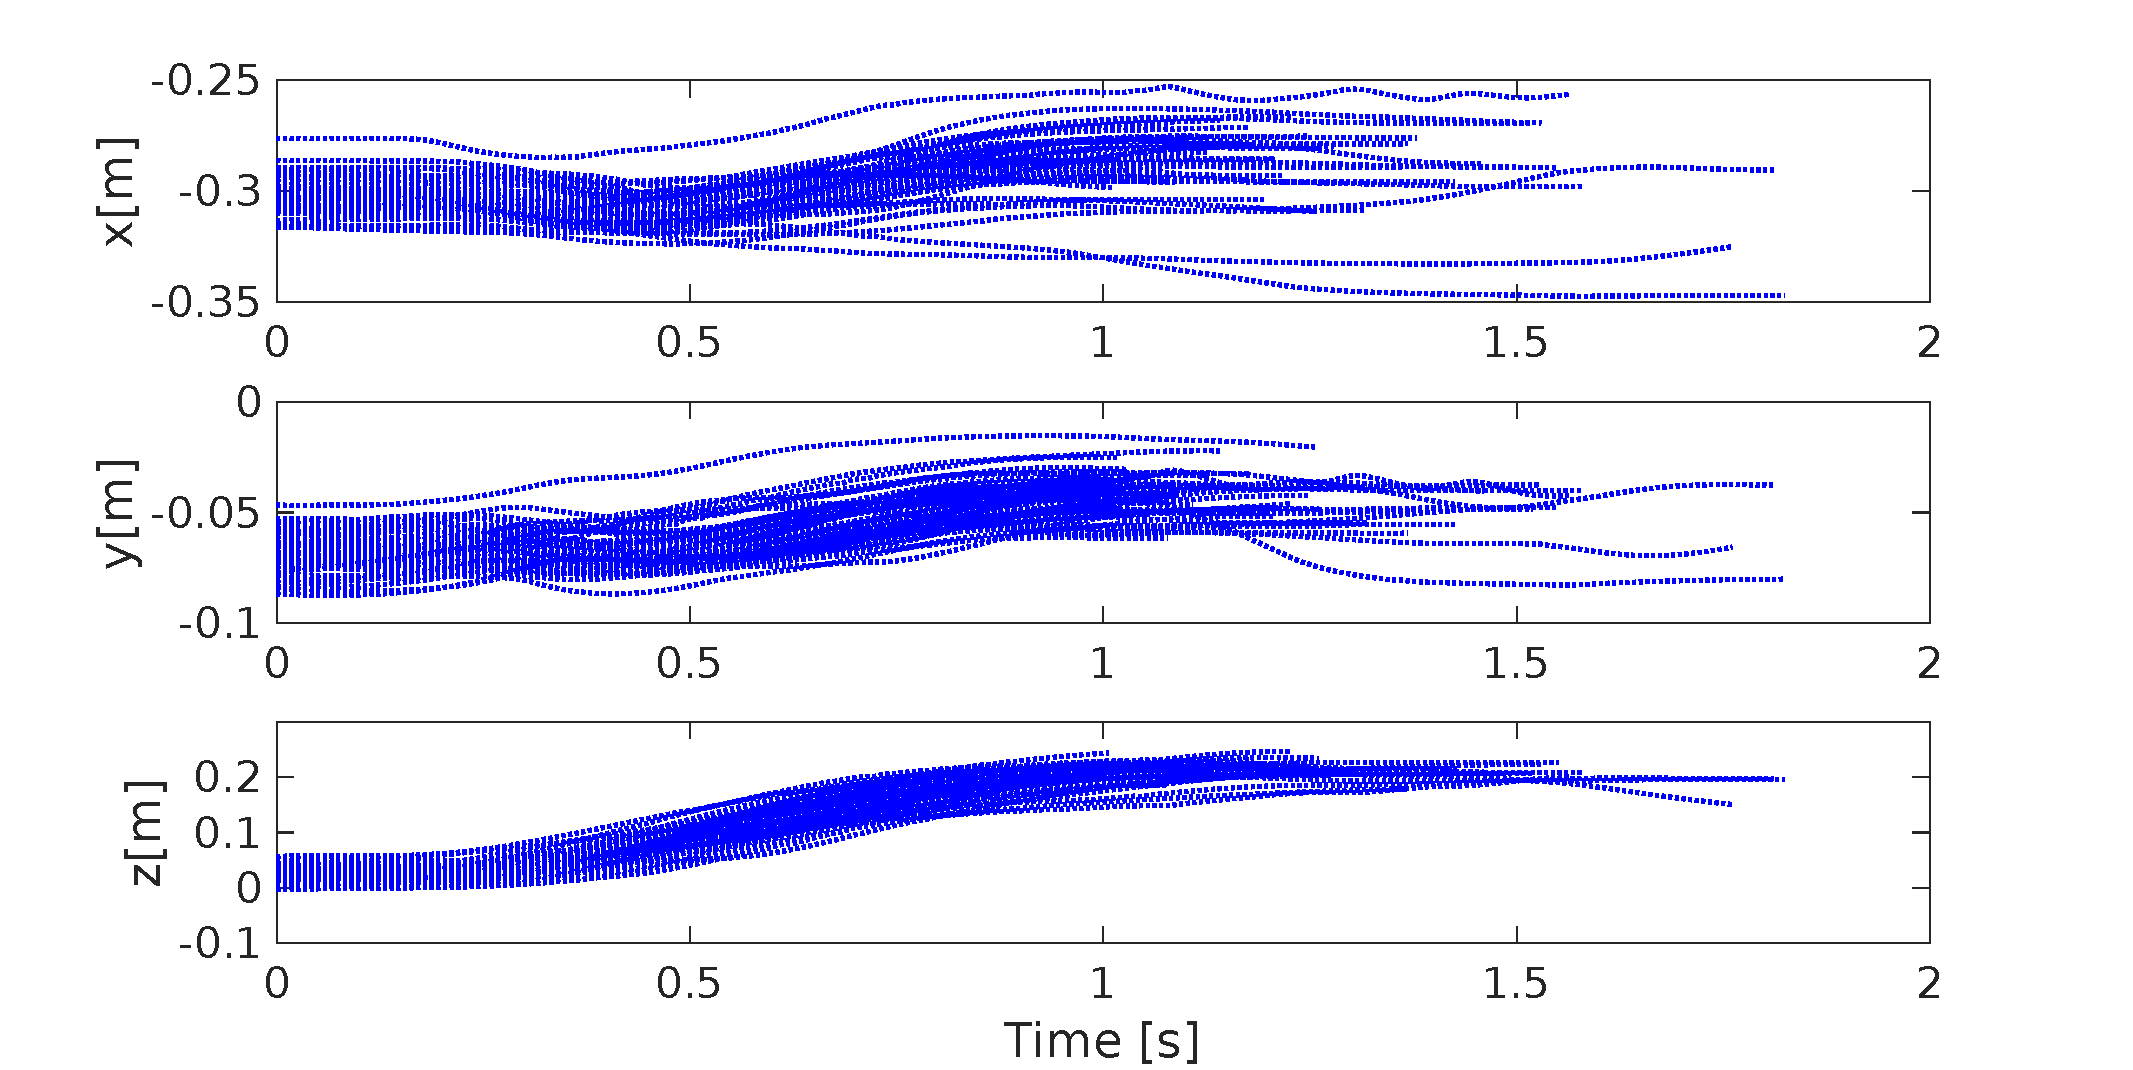
\includegraphics[height=7cm]{figs/geomagic_lifting_trajectories.pdf}
\caption{Some trajectories recorded when the geomagic is used to lift the left arm: Cartesian position of the end-effector.}
\label{fig:trajectories}
\end{figure}

Demonstrated trajectories and their corresponding forces can be recorded directly from the robot, by accessing the Cartesian interface and the Cartesian end-effector wrench computed by \textit{wholeBodyDynamicsTree}.



 
%%%%%%%%%%%%%%%%%%%%%%%%%%%%%%%%%%%%%%%%%%%%%%%%%%%%%%%%%%%%%%%%%%%%%%%


\subsection{Learning a ProMP of the lifting movement}

Once we record a set of trajectories, we can learn the distribution of these demonstration in the form of a probabilistic movement primitive (ProMP) \cite{Paraschos_NIPS_2013a}.
Our toolbox for generating the proMP is currently written in Matlab, and available at \url{https://github.com/inria-larsen/icubLearningTrajectories}.

Let us consider the $n$ recorded trajectories \textcircled{$ \tau$} $= \{\tau_1,..., \tau_n \}$, where  the $i$-th trajectory is $\tau_i = \{y(t_1), ..., y(t_{f_i})\}$. 
$y(t)$ is the vector containing all the variables used to learn the ProMP, the simplest case being the mono-dimensional ProMP. If we want to learn the ProMP of the lifting motion (see Figure \ref{fig:trajectories}), the simplest case is $y(t) =\begin{bmatrix} z\end{bmatrix}^{\top}$, that is the $z$-axis Cartesian coordinate of the end-effector. You may notice that the duration of all the trajectories can be different, i.e.,  $t_{f_i}$ may be variable across demonstrations. 
To be able to find a common representation in term of primitive, a temporal modulation of the trajectories is applied, such that they all have the same number of samples $\bar{s}$. 

The ProMP is a Bayesian parametric model of the demonstrated trajectories in the form: 
$$y(t) = \Phi(t)^\top \omega + \epsilon_y$$ 
where $\Phi$ are $m$ radial basis functions scattered across time, scaled by the parameters vector $\omega \in R^m$. 
$\epsilon_y \sim \mathcal{N}(0, \beta) $ is the trajectory noise. 

For each $i$-th trajectory $\tau_i$, we compute the $\omega_i$ parameters vector:
$$y_i(t) = \Phi(t)^\top \omega_i + \epsilon_y$$ 
by minimizing the error between the observed trajectory $y_i(t)$ and its model $\Phi(t)^\top \omega_i + \epsilon_y$. This is done using the Least Mean Square algorithm, i.e.:
$$ \omega_i = (\Phi(t)^\top\Phi(t))^{-1}\Phi(t)^\top y_i(t).$$

Then, using the aggregated $[\omega_1,..., \omega_n]$ parameters, we can compute the distribution over these parameters $\omega \sim \mathcal{N}(\mu_\omega, \Sigma_w)$, and from this distribution, compute the distribution of the observed trajectories, which is the ProMP.

Figure \ref{fig:proMPlifting} shows the ProMP for the lifting motion, computed with the number of reference samples $\bar{s}=100$, number of basis functions $m=5$; the center of each RBF is equally distributed between 1 and $\bar{s}$.


\begin{figure}[h]
\centering
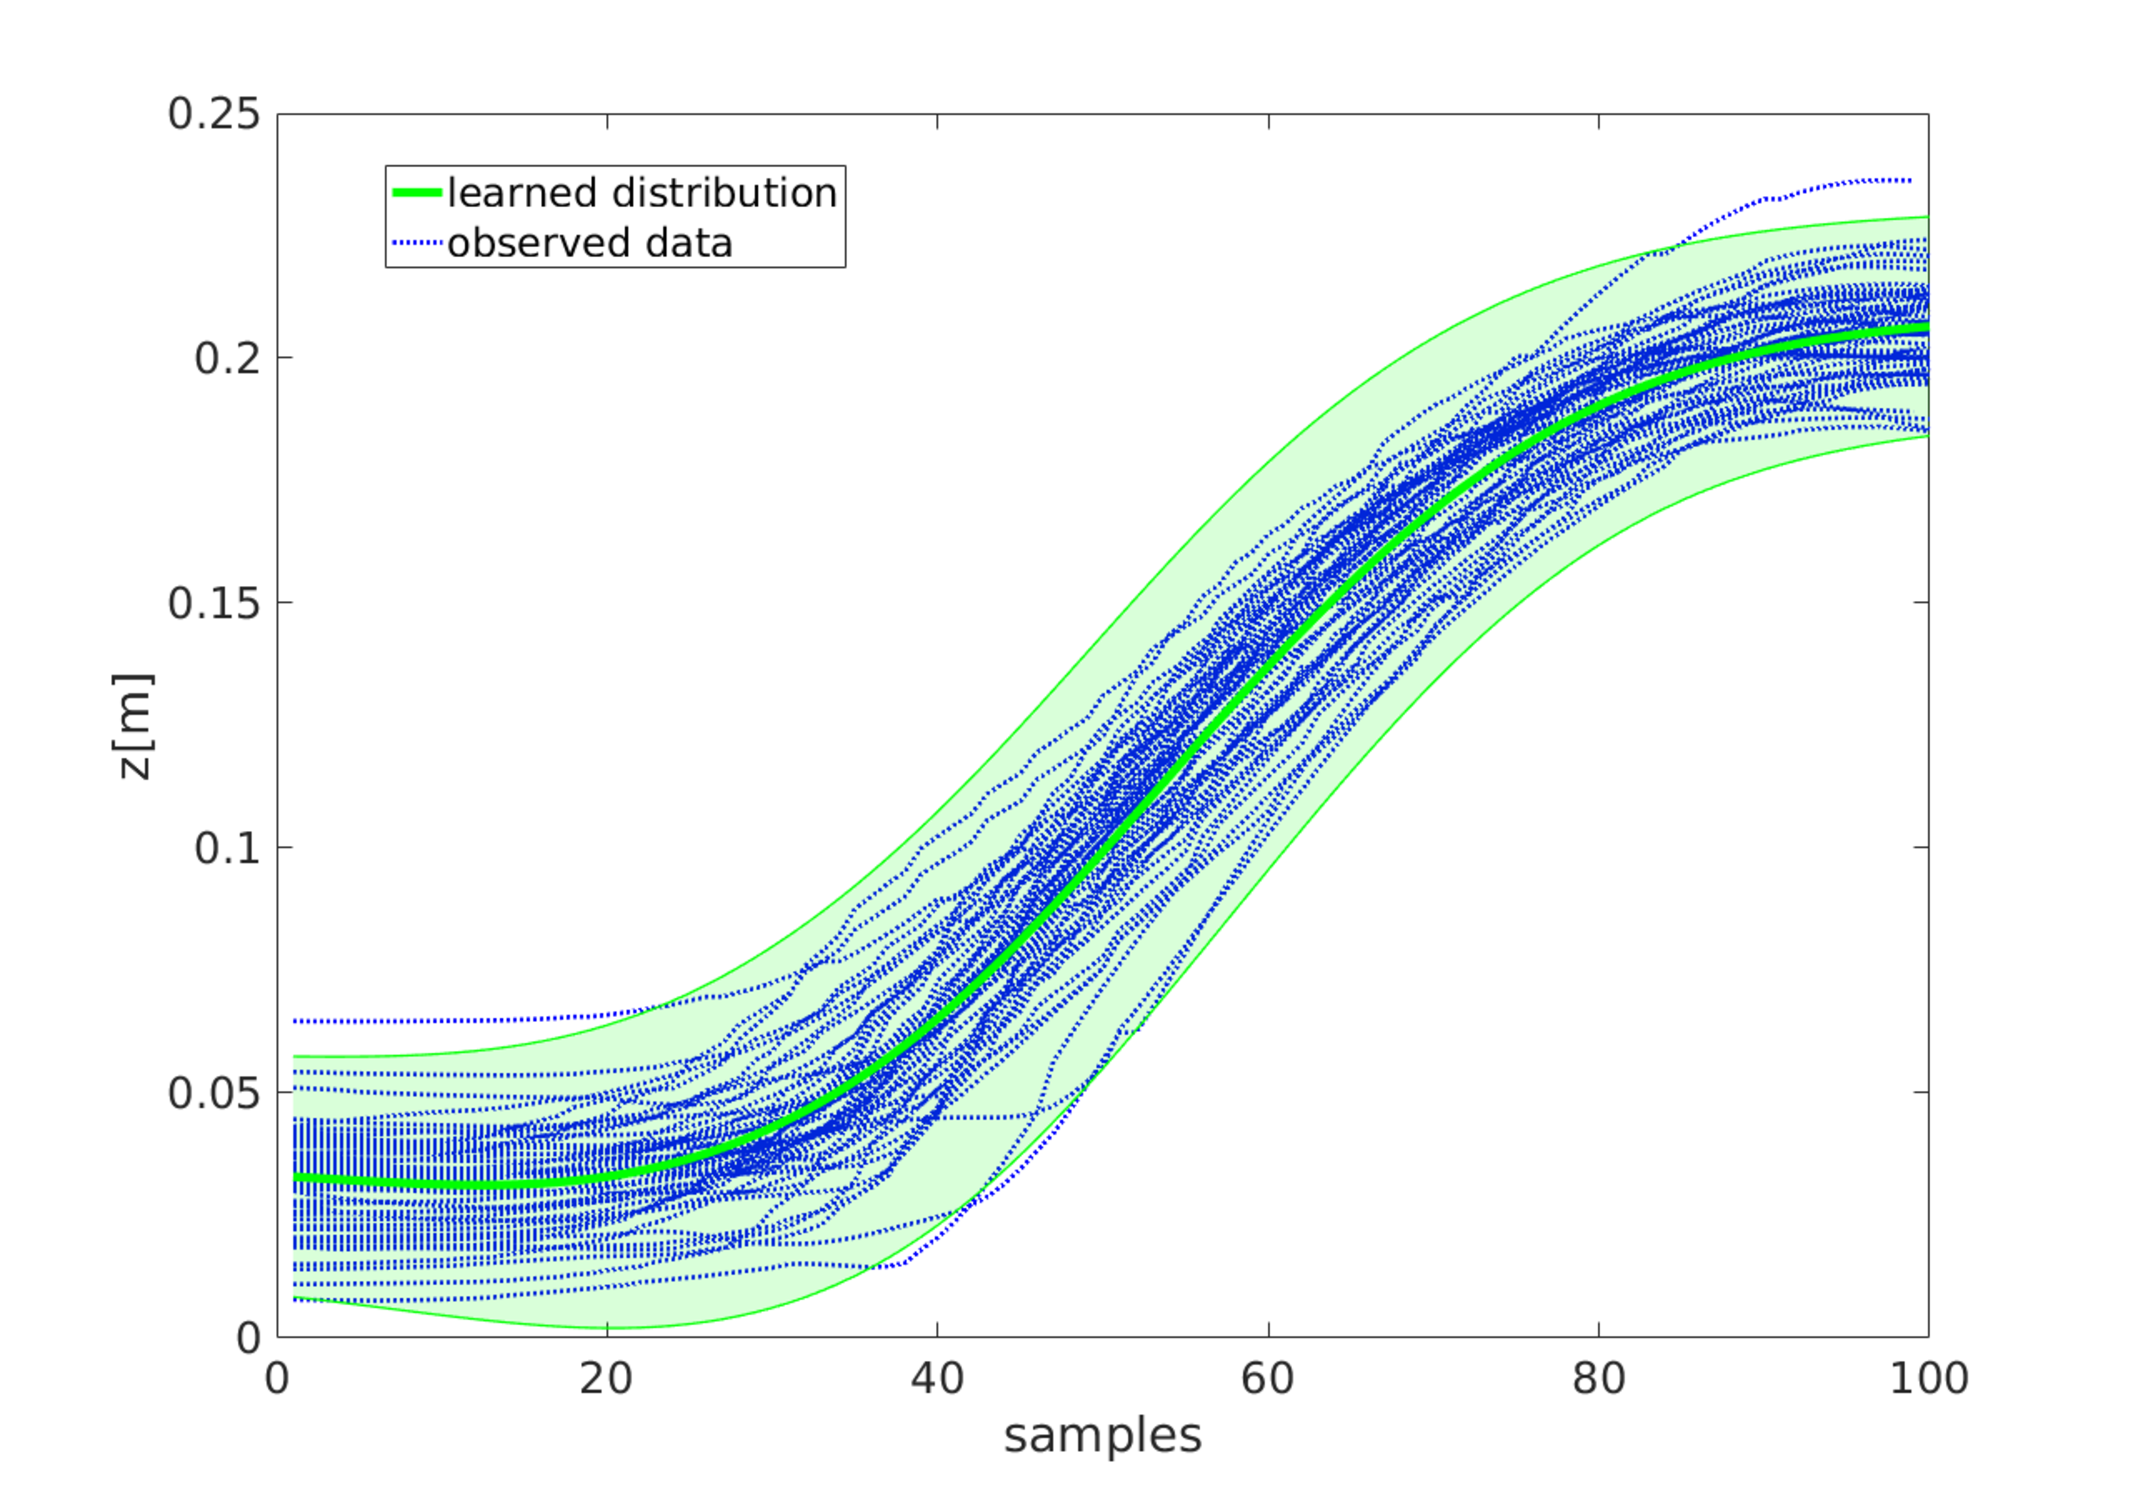
\includegraphics[height=9cm]{figs/proMPz.pdf}
\caption{proMP of the left end-effector $z$ coordinate when the arm is being lifted.}
\label{fig:proMPlifting}
\end{figure}





%%%%%%%%%%%%%%%%%%%%%%%%%%%%%%%%%%%%%%%%%%%%%%%%%%%%%%%%%%%%%%%%%%%%%%%
\subsection{Predicting the movement from initial observations}

Once the ProMP of a certain gesture has been learned (i.e., we have computed $\omega$ from $\omega_1, \ldots, \omega_n$), we can use it to predict the evolution of a movement just after few observations. Of course, the underlying hypothesis is that the movement that is observed ``belongs" to the distribution of demonstrated trajectories.

Let us consider the ProMP with the parameters distribution $\omega \sim \mathcal{N}(\mu_\omega, \Sigma_\omega)$.  

Suppose that we have $n_o$ observations of the trajectory to predict (e.g., lifting the arm), called 
$$D=[y^o(t_1),\ldots, y^o(t_{n_o})].$$

Our goal is to predict the evolution of the trajectory after $t_{n_o}$, i.e., find $\hat{y}(t_{n_o+1}),\ldots,\hat{y}(\hat{t}_f)$, where $\hat{t}_f$ is the estimate of the trajectory duration (by default the mean of all the $t_{f_1}, \ldots, t_{f_n}$). 
This is equivalent to predicting the entire trajectory $\hat{\tau}$ where the first $n_o$ samples are known and equal to the observations: $\hat{\tau} = \{y^o(t_{1}), ..., y^o(t_{n_o}), \hat{y}(t_{n_o+1}), ..., \hat{y}(t_{\hat{t}_f})\}$.
Therefore, our prediction problem consists in predicting $\hat{\tau}$ given the $D$ observations. Since $\hat{\tau}$ is computed by a ProMP, finding $\hat{\tau}$ means finding the $\hat{\omega}$ generating the  $\hat{\tau}$, by:
$$\left\{
\begin{array}{rl}
\hat{\mu}_\omega &= \mu_\omega + K(D - \Phi_t^\top \mu_\omega) \\ 
\hat{\Sigma}_\omega &= \Sigma_\omega - K(\Phi_t^\top \Sigma_\omega) \\
K&= \Sigma_\omega\Phi_t^\top(\Sigma_D + \Phi_t^\top\Sigma_\omega \Phi_t)^{-1}
\end{array}
\right.$$

Figure \ref{fig:predictionLifting15} shows the predicted trajectory for the lifting motion of the left arm of iCub after $n_{o}=15$. An example of the predicted trajectory for lifting the arm in Gazebo can be seen here: \url{https://www.youtube.com/watch?v=0i5O4Lsf7Jc&feature=youtu.be}.


\begin{figure}[h]
\centering
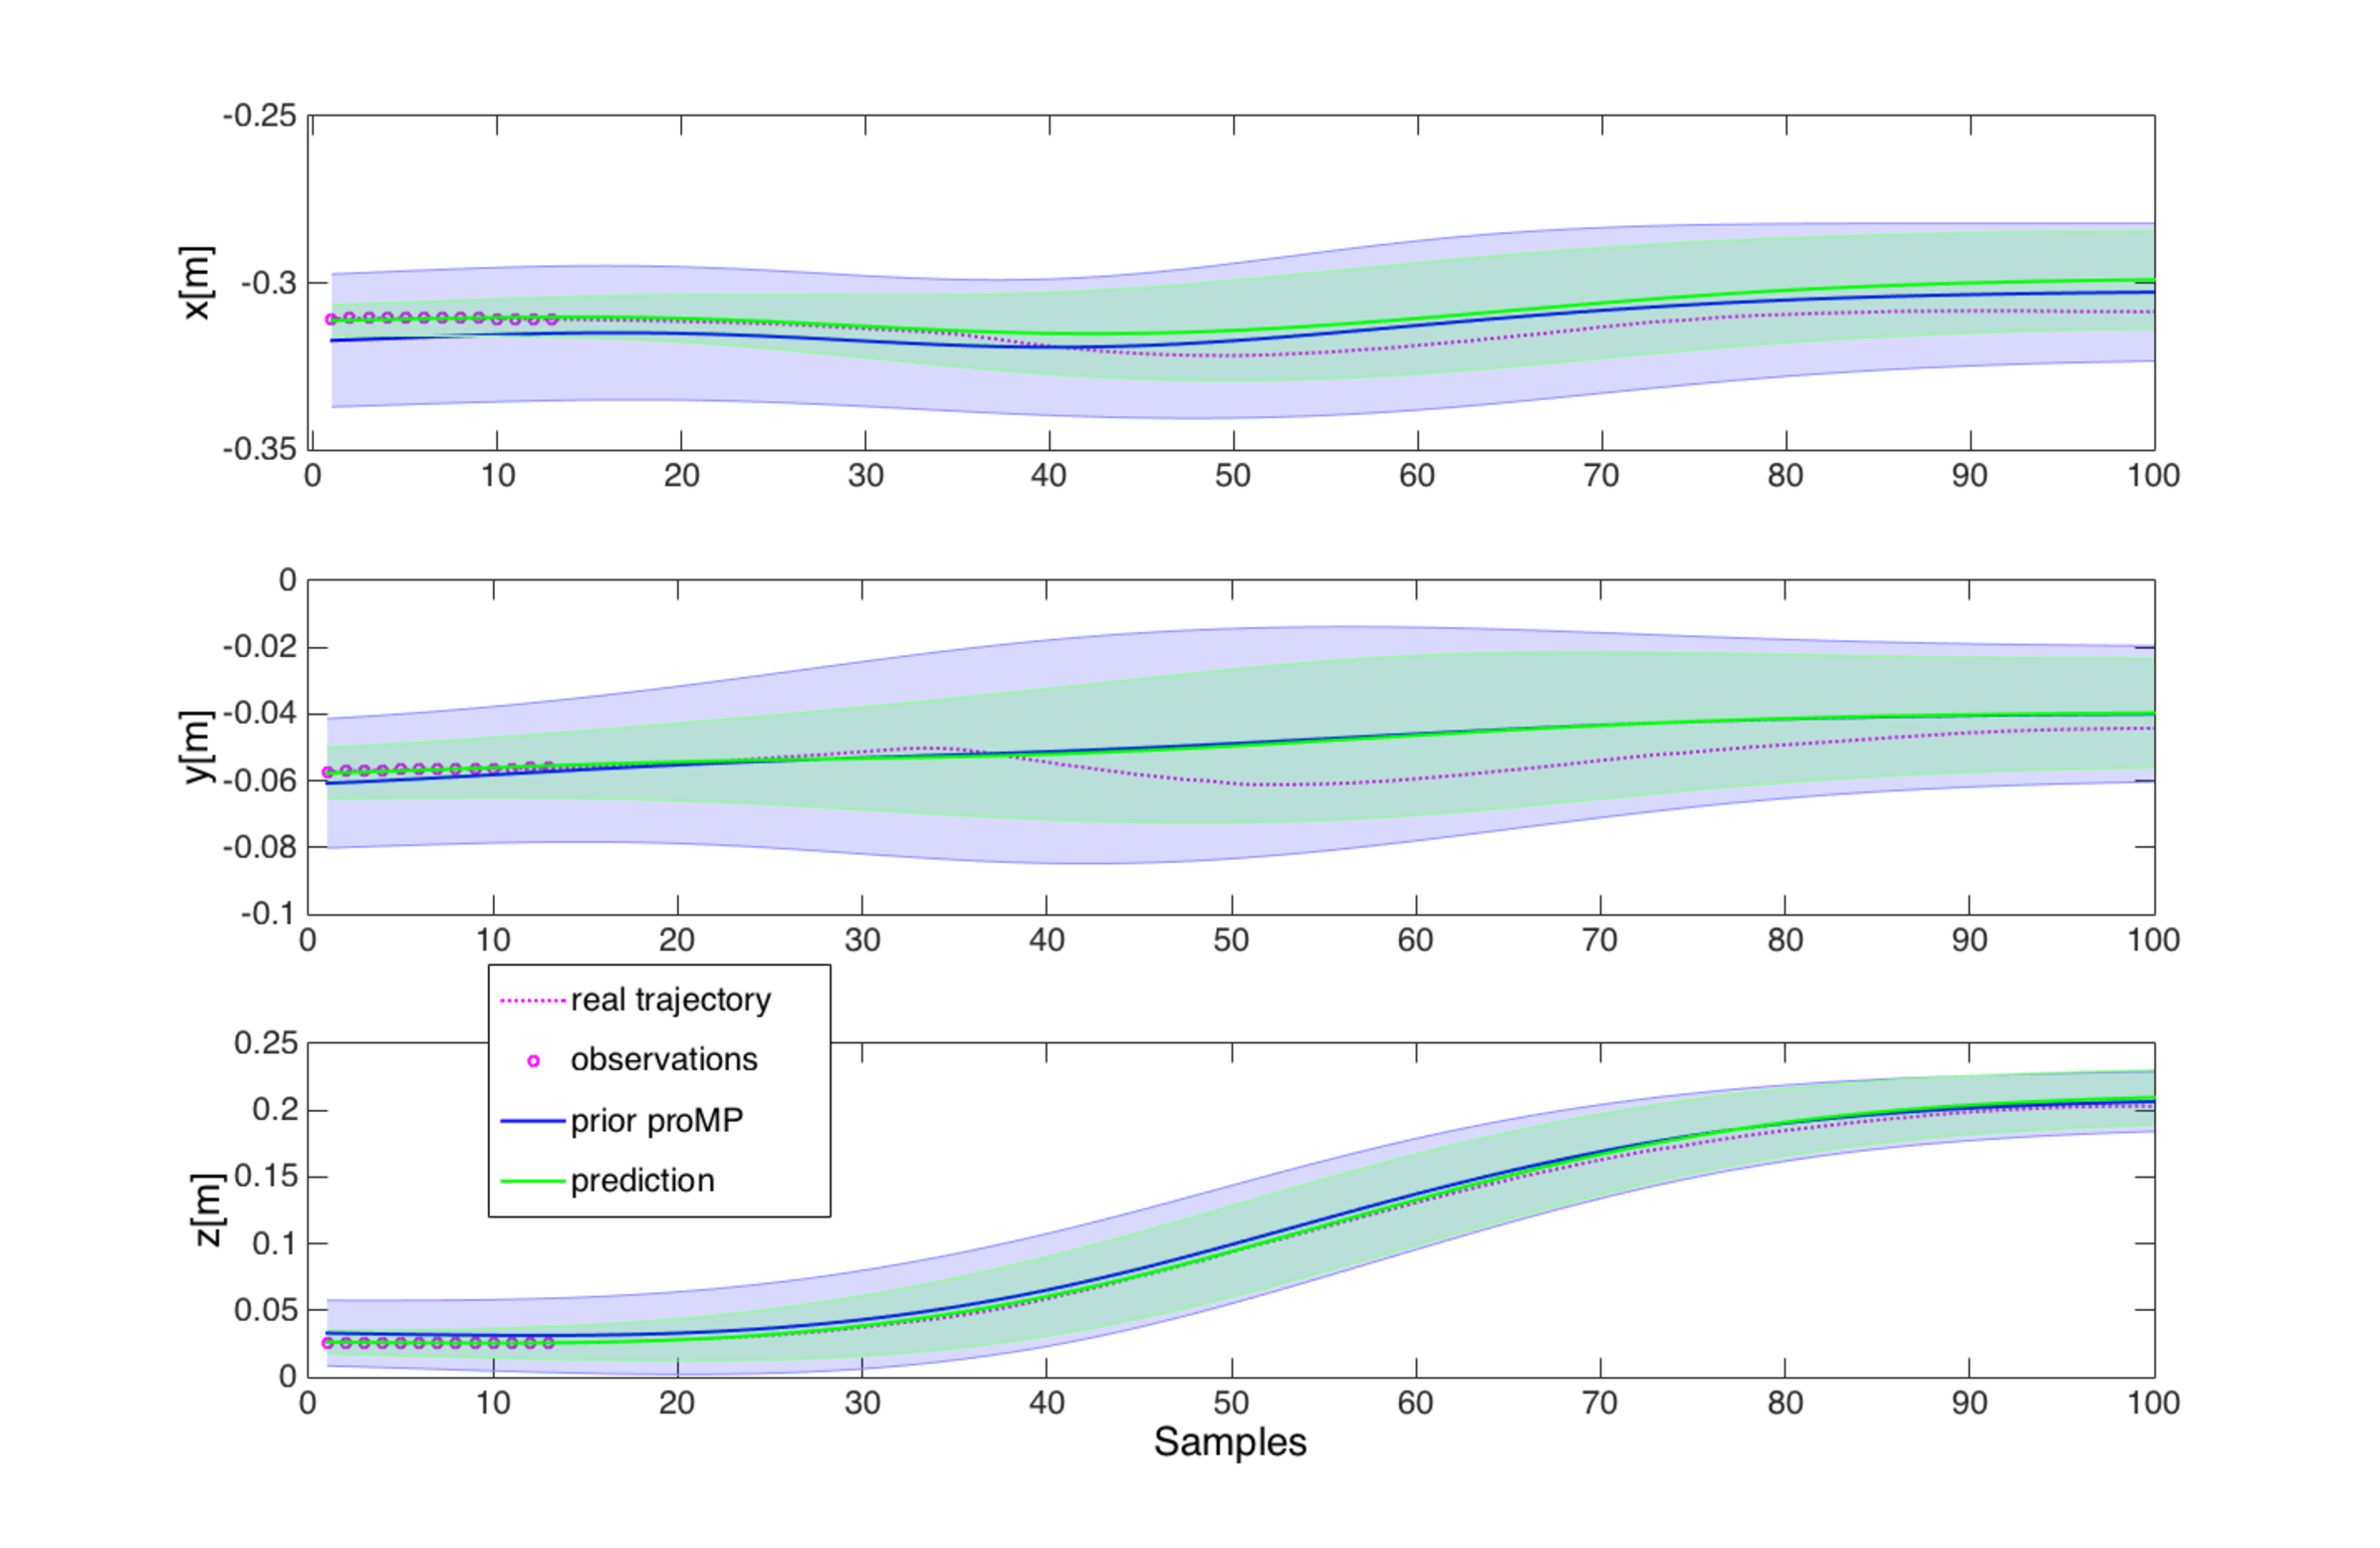
\includegraphics[height=11cm]{figs/proMP_prediction.pdf}
\caption{Prediction of the future trajectory, after $n_o=15$ observations, given the prior proMP learned from $n$ demonstrations.}
\label{fig:predictionLifting15}
\end{figure}









